\documentclass[journal,10pt]{IEEEtran}

\usepackage[utf8]{inputenc}
\usepackage{graphicx}
\usepackage{booktabs}
\usepackage{multirow}
\usepackage{xcolor}
\usepackage[colorlinks=false, pdfborder={0 0 0}]{hyperref}
\usepackage{amsmath}
\usepackage{balance}
\usepackage{tikz}
\usetikzlibrary{positioning, arrows.meta, shapes.geometric, fit, backgrounds, calc, decorations.pathreplacing}

% TODO markers (keep for remaining gaps)
\newcommand{\todo}[1]{\textcolor{red}{\textbf{[TODO: #1]}}}
\newcommand{\fixme}[1]{\textcolor{orange}{\textbf{[FIXME: #1]}}}

\title{A Systematic Survey of CXL Type-3 Devices:\\ Evolution, Architectures, and Future Directions\\ for Memory-Intensive Computing}

\author{\IEEEauthorblockN{Dawen Liang}
\IEEEauthorblockA{\textit{College of Engineering and Computer Science}\\
\textit{Syracuse University}\\
Syracuse, NY, USA\\
dliang02@hotmail.com}
}

\begin{document}

\maketitle

\begin{abstract}
The rapid growth of memory-intensive workloads, such as trillion-parameter language models and in-memory databases that process petabytes of data, has revealed fundamental limitations in traditional memory architectures. Compute Express Link (CXL), a cache-coherent interconnect built on PCIe, introduces Type-3 memory expanders. These expanders create a new layer between local DRAM and storage, providing byte-addressable, load/store-accessible capacity with a latency of 200 to 400 nanoseconds. This survey examines CXL Type-3 devices in three areas: (1)~hardware architecture and performance, (2)~systems software including kernel-level tiering, allocation, and virtualization support, and (3)~emerging applications in in-memory databases, high-performance computing, and AI/LLM workloads. We review over 40 papers from respected venues (OSDI, ASPLOS, MICRO, SIGMOD, SOSP) published from 2022 to 2025 and highlight key challenges such as managing tail latency, ensuring security in shared memory pools, and exploring hardware-software co-design opportunities. By connecting the systems and machine learning communities, we assert that CXL Type-3 devices are crucial for the next generation of memory-intensive computing systems.
\end{abstract}

\begin{IEEEkeywords}
CXL, Compute Express Link, Type-3 devices, memory disaggregation, memory-intensive computing, memory tiering
\end{IEEEkeywords}

%% ============================================================
%% SECTION 1: INTRODUCTION
%% ============================================================
\section{Introduction}
\label{sec:intro}

Modern datacenter workloads often face memory bottlenecks rather than computation delays. Barroso et al.\ identified a critical latency range, called ``killer microseconds,'' where operations taking 1 to 100 microseconds---including remote memory accesses and inter-socket communication---become the primary performance limitation in large systems~\cite{barrosoAttackKillerMicroseconds2017}. This challenge has escalated significantly: large language models now need hundreds of gigabytes to terabytes of parameter storage, in-memory databases require increasingly larger buffer pools, and graph analytics workflows frequently surpass the memory capacity of a single server.

Compute Express Link (CXL) has emerged as a transformative technology to tackle this memory capacity issue. Built on the PCIe physical layer, CXL enables cache-coherent, byte-addressable access to external memory devices through its CXL.mem protocol~\cite{CXL3.1,CXL4.0}. Unlike previous disaggregation methods using RDMA or network-attached storage, CXL Type-3 memory expanders allow CPUs to access remote DRAM using native load/store instructions with latencies of 200 to 400 nanoseconds---about 2 to 3 times that of local DRAM, compared to the 10 to 100 times penalty of network-based solutions. The concept of disaggregated memory was first systematically examined by Lim et al., who showed that separating memory from compute blades could achieve 50\% better performance per dollar for datacenter workloads~\cite{limSystemlevelImplicationsDisaggregated2012}.

The systems and application communities have quickly converged on CXL as the enabling technology for memory-intensive computing. Database systems now use CXL for unified buffer pools across multiple compute nodes~\cite{10.1145/3722212.3724460,huang2025tigon}; operating systems have added CXL-aware tiering into the Linux kernel~\cite{marufTPPTransparentPage2023}; and AI researchers are designing memory-augmented architectures that naturally align with CXL's features~\cite{chengConditionalMemoryScalable2026}. A recent competing survey by Chen et al.~\cite{chen2025nextgencomputingsystemscompute} looks at CXL from a broad protocol viewpoint; our work is distinct as it specifically focuses on Type-3 devices and their applications in memory-intensive computing, especially at the emerging intersection of CXL and AI.

This survey addresses four research questions: \textbf{RQ1:} What are the performance characteristics of real CXL Type-3 hardware? \textbf{RQ2:} How has systems software adapted to leverage CXL memory tiering? \textbf{RQ3:} Which application areas benefit the most from CXL Type-3 devices? \textbf{RQ4:} What are the key challenges for CXL adoption?

The rest of this paper is organized as follows. Section~\ref{sec:background} provides background on CXL protocols and the evolution of memory disaggregation. Section~\ref{sec:hardware} explores CXL hardware architecture and performance. Section~\ref{sec:software} reviews systems software support. Section~\ref{sec:apps} analyzes applications in databases, high-performance computing, and AI workloads. Section~\ref{sec:challenges} discusses open challenges, and Section~\ref{sec:conclusion} concludes.


%% ============================================================
%% SECTION 2: BACKGROUND
%% ============================================================
\section{Background}
\label{sec:background}

\subsection{CXL Protocol Overview}
\label{sec:bg-protocol}

CXL defines three sub-protocols operating over a shared PCIe physical link: \textit{CXL.io} provides PCIe-compatible I/O semantics for device discovery and configuration; \textit{CXL.cache} enables devices to cache host memory with hardware-managed coherence; and \textit{CXL.mem} allows hosts to access device-attached memory using load/store instructions with full cache coherence~\cite{CXL3.1}. Devices fall into three types based on protocol usage: Type-1 devices (accelerators using CXL.io and CXL.cache), Type-2 devices (accelerators with their own memory using all three protocols), and Type-3 devices (memory expanders using CXL.io and CXL.mem). This survey focuses only on Type-3 devices, which are fundamental for CXL-based memory disaggregation.

CXL's specification has rapidly evolved. CXL~1.0 and 1.1 established single-device attachment over PCIe~5.0. CXL~2.0 introduced memory pooling using CXL switches, allowing multiple hosts to share a common memory pool. CXL~3.0 further enhanced the fabric with multi-level switching and back-invalidation snooping for improved coherence scalability~\cite{CXL3.1}. The latest CXL~4.0 specification doubles the data rate to 128\,GT/s on a PCIe~7.0 physical layer, achieving up to 768\,GB/s unidirectional bandwidth per x16 link, and introduces native support for multi-rack topologies along with enhanced memory RAS features~\cite{CXL4.0}.


\subsection{Type-3 Device Positioning in the Memory Hierarchy}
\label{sec:bg-hierarchy}

CXL Type-3 devices create a new tier in the memory hierarchy, as illustrated in Fig.~\ref{fig:memory_hierarchy}. Sun et al.\ measured genuine CXL memory systems and found that CXL DRAM access latencies range from 1.35 to 3 times higher than local DDR, depending on how mature the implementation is~\cite{10.1145/3613424.3614256}. At the system level, CXL memory acts as a CPU-less NUMA node: it is byte-addressable and can be accessed using standard load/store instructions, though it has different latency and bandwidth characteristics than local DRAM.

This placement---between local DRAM (about 100\,ns) and NVMe storage (about 10 to 100\,$\mu$s)---makes CXL Type-3 memory especially suitable for workloads needing large capacity but less sensitivity to latency. The host processor's hardware prefetcher can utilize CXL memory, and existing NUMA-aware allocation policies can be applied for page placement, allowing applications to migrate without requiring code changes.

%% ---- FIGURE 1: Memory Hierarchy ----
\begin{figure}[t]
\centering
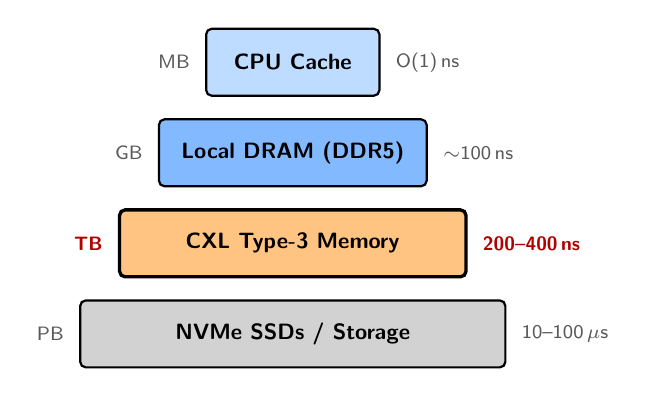
\begin{tikzpicture}[
    tier/.style={draw, rectangle, rounded corners=2pt, minimum height=0.85cm,
                 text centered, font=\sffamily\footnotesize, thick},
    anno/.style={font=\sffamily\scriptsize, text=gray!70!black},
    brace/.style={decorate, decoration={brace, amplitude=4pt, raise=2pt}},
]

% Color definitions
\definecolor{cacheC}{RGB}{190,220,255}
\definecolor{dramC}{RGB}{130,185,255}
\definecolor{cxlC}{RGB}{255,195,130}
\definecolor{nvmeC}{RGB}{210,210,210}

% Tiers (narrower to fit single column)
\node[tier, fill=nvmeC, minimum width=5.4cm] (nvme) at (0,0)
  {\textbf{NVMe SSDs / Storage}};
\node[tier, fill=cxlC, minimum width=4.4cm, line width=1.2pt] (cxl) at (0,1.15)
  {\textbf{CXL Type-3 Memory}};
\node[tier, fill=dramC, minimum width=3.4cm] (dram) at (0,2.3)
  {\textbf{Local DRAM (DDR5)}};
\node[tier, fill=cacheC, minimum width=2.2cm] (cache) at (0,3.45)
  {\textbf{CPU Cache}};

% Latency annotations (right side)
\node[anno, right=2pt] at (cache.east) {O(1)\,ns};
\node[anno, right=2pt] at (dram.east)  {$\sim$100\,ns};
\node[anno, right=2pt, text=red!70!black, font=\sffamily\scriptsize\bfseries] at (cxl.east)
  {200--400\,ns};
\node[anno, right=2pt] at (nvme.east)  {10--100\,$\mu$s};

% Capacity annotations (left side)
\node[anno, left=2pt] at (cache.west) {MB};
\node[anno, left=2pt] at (dram.west)  {GB};
\node[anno, left=2pt, text=red!70!black, font=\sffamily\scriptsize\bfseries] at (cxl.west)
  {TB};
\node[anno, left=2pt] at (nvme.west)  {PB};

\end{tikzpicture}
\caption{The expanded memory hierarchy with CXL Type-3 devices. CXL introduces a critical intermediate tier that bridges the ``killer microsecond'' capacity-latency gap between direct-attached DRAM and block storage. Latency and capacity values are representative ranges from real hardware measurements~\cite{10.1145/3613424.3614256,weisgut2025cxl}.}
\label{fig:memory_hierarchy}
\end{figure}


\subsection{Pre-CXL Disaggregation: The Evolutionary Path}
\label{sec:bg-precxl}

The idea of memory disaggregation has deep roots that predate CXL. Lim et al.\ first proposed this concept at ISCA~2009~\cite{10.1145/1555754.1555789}, imagining ``memory blades'' connected through a high-speed interconnect. They later developed a software prototype on the Xen hypervisor, showing that disaggregated memory with microsecond-level latency (4\,$\mu$s over PCIe~2.0) could achieve performance equivalent to all-local memory setups while offering 50\% better performance per dollar~\cite{limSystemlevelImplicationsDisaggregated2012}. This research established crucial design principles, including the need for simple page replacement policies at microsecond latencies and the beneficial interaction between disaggregated memory and content-based page sharing, both of which remain relevant for CXL system design today.

Klimovic et al.\ extended disaggregation to flash storage, demonstrating that remote flash accessed via 10\,GbE with iSCSI could reduce application-level throughput by only 20\%, with a 260\,$\mu$s latency acceptable for workloads with millisecond-scale SLAs~\cite{klimovicFlashStorageDisaggregation2016}. This work highlighted the key tension between the benefits of disaggregation (like improved utilization and independent scaling) and the network overhead that later drove the need for the CXL interconnect.

Gao et al.\ took disaggregated memory further with Clio, a hardware-software co-designed system featuring custom CBoards with ASIC-accelerated pathways and ARM-based control systems~\cite{10.1145/3503222.3507762}. Clio achieved bounded lookup latency by using overflow-free hash-based page tables and showed that disaggregated memory nodes benefit from separating fast-path data operations (handled by hardware) from slow-path metadata management (managed by software). CXL Type-3 devices incorporate many of these design lessons while removing the need for custom network protocols by utilizing the PCIe physical layer.


\subsection{Workload-Driven Demand for CXL}
\label{sec:bg-workload}

Three application areas have driven the demand for CXL Type-3 memory. In-memory databases like SAP HANA have shown that CXL memory expansion allows processing of datasets larger than available DRAM with acceptable performance loss~\cite{ahn2024examination}. Billion-scale nearest neighbor search services, such as CXL-ANNS, require over 40\,TB of index memory across multiple devices, making CXL pooling crucial for cost-effective deployment~\cite{jang2023cxl}. Recently, memory-augmented LLM architectures like Engram have introduced enormous parameter tables (with over 100 billion entries) featuring deterministic, prefetchable access patterns that naturally fit CXL's byte-addressable memory design~\cite{chengConditionalMemoryScalable2026}. These converging demands from the database, systems, and AI communities encourage a unified examination of CXL Type-3 devices.


%% ============================================================
%% SECTION 3: CXL HARDWARE
%% ============================================================
\section{CXL Hardware Architecture and Performance}
\label{sec:hardware}

\subsection{HDM Models, MLD, and Multi-Headed Devices}
\label{sec:hw-hdm}

The CXL specification defines Host-managed Device Memory (HDM) as the main abstraction for Type-3 device memory. HDM supports three decoder models: HDM-H (host-only decoding), HDM-D (device-managed decoding), and HDM-DB (device-managed with back-invalidation)~\cite{CXL3.1}. Starting with CXL~2.0, Multi-Logical Devices (MLDs) allow a single physical device to present up to 16 logical devices, each assignable to different hosts. This feature, along with CXL switches that support fabric-level pooling, supports rack-scale memory sharing. Multiple hosts can allocate and release memory from a shared pool. Fig.~\ref{fig:cxl_topology} illustrates how CXL topologies have changed from direct attachment to multi-rack fabrics.

Pond, the first CXL-based memory pooling system designed for production cloud environments, showed that small-scale pooling across 8--16 sockets can recover up to 25\% of stranded DRAM while introducing only 70--90\,ns of added latency~\cite{liPondCXLBasedMemory2022}. Pond introduced a Zero-CPU NUMA Node (zNUMA) abstraction that presents pooled CXL memory as a NUMA node without linked CPU cores. This allows the OS to use its existing NUMA allocation policies. DRack expanded pooling to the rack scale, combining CXL memory pooling with NIC pooling to tackle inter-rack communication issues~\cite{zhang2025drack}. DRack's design demonstrated that the blend of memory-semantic access (CXL.mem) and device pooling (CXL switches) could resolve both memory stranding and network underutilization issues.

%% ---- FIGURE 2: CXL Topology Evolution ----
\begin{figure*}[t]
\centering
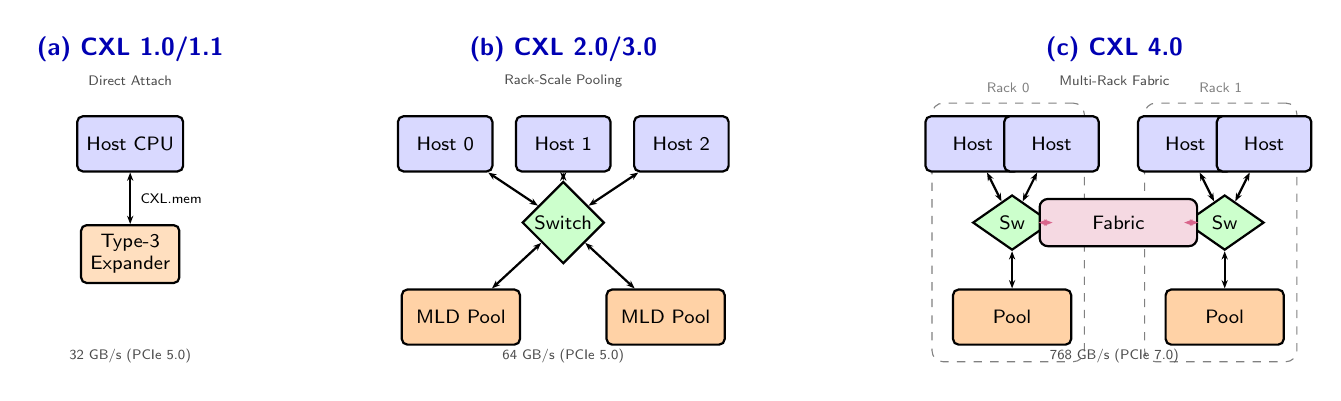
\begin{tikzpicture}[
    host/.style={draw, fill=blue!15, rectangle, rounded corners=2pt,
                 minimum width=1.2cm, minimum height=0.7cm, font=\sffamily\scriptsize, thick},
    mem/.style={draw, fill=orange!25, rectangle, rounded corners=2pt,
                minimum width=1.2cm, minimum height=0.7cm, font=\sffamily\scriptsize, thick, align=center},
    sw/.style={draw, fill=green!20, diamond, minimum width=1.0cm,
               minimum height=0.7cm, font=\sffamily\scriptsize, thick, inner sep=1pt},
    mld/.style={draw, fill=orange!35, rectangle, rounded corners=2pt,
                minimum width=1.5cm, minimum height=0.7cm, font=\sffamily\scriptsize, thick},
    fabric/.style={draw, fill=purple!15, rectangle, rounded corners=3pt,
                   minimum width=2.0cm, minimum height=0.6cm, font=\sffamily\scriptsize, thick},
    link/.style={thick, -{Stealth[length=3pt]}},
    bilink/.style={thick, {Stealth[length=3pt]}-{Stealth[length=3pt]}},
    phase/.style={font=\sffamily\small\bfseries, text=blue!70!black},
    sub/.style={font=\sffamily\tiny, text=gray!60!black},
]

% === (a) CXL 1.0/1.1: Direct Attach ===
\node[phase] at (0, 3.2) {(a) CXL 1.0/1.1};
\node[sub] at (0, 2.8) {Direct Attach};

\node[host] (h1a) at (0, 2.0) {Host CPU};
\node[mem]  (m1a) at (0, 0.6) {Type-3\\Expander};
\draw[bilink] (h1a) -- (m1a) node[midway, right, font=\sffamily\tiny] {CXL.mem};

% === (b) CXL 2.0/3.0: Rack-Scale Pooling ===
\node[phase] at (5.5, 3.2) {(b) CXL 2.0/3.0};
\node[sub] at (5.5, 2.8) {Rack-Scale Pooling};

\node[host] (h1b) at (4.0, 2.0) {Host 0};
\node[host] (h2b) at (5.5, 2.0) {Host 1};
\node[host] (h3b) at (7.0, 2.0) {Host 2};
\node[sw]   (sw1) at (5.5, 1.0) {Switch};
\node[mld]  (mld1) at (4.2, -0.2) {MLD Pool};
\node[mld]  (mld2) at (6.8, -0.2) {MLD Pool};

\draw[bilink] (h1b) -- (sw1);
\draw[bilink] (h2b) -- (sw1);
\draw[bilink] (h3b) -- (sw1);
\draw[bilink] (sw1) -- (mld1);
\draw[bilink] (sw1) -- (mld2);

% === (c) CXL 4.0: Multi-Rack Fabric ===
\node[phase] at (12.5, 3.2) {(c) CXL 4.0};
\node[sub] at (12.5, 2.8) {Multi-Rack Fabric};

% Rack 0
\begin{scope}[on background layer]
\node[draw, dashed, gray, rounded corners=4pt, fit={(10.3,-0.65) (12.0,2.4)},
      label={[font=\sffamily\tiny, text=gray]above:Rack 0}] {};
\end{scope}
\node[host] (h1c) at (10.7, 2.0) {Host};
\node[host] (h2c) at (11.7, 2.0) {Host};
\node[sw]   (sw2) at (11.2, 1.0) {Sw};
\node[mld]  (mp1) at (11.2, -0.2) {Pool};
\draw[bilink] (h1c) -- (sw2);
\draw[bilink] (h2c) -- (sw2);
\draw[bilink] (sw2) -- (mp1);

% Rack 1
\begin{scope}[on background layer]
\node[draw, dashed, gray, rounded corners=4pt, fit={(13.0,-0.65) (14.7,2.4)},
      label={[font=\sffamily\tiny, text=gray]above:Rack 1}] {};
\end{scope}
\node[host] (h3c) at (13.4, 2.0) {Host};
\node[host] (h4c) at (14.4, 2.0) {Host};
\node[sw]   (sw3) at (13.9, 1.0) {Sw};
\node[mld]  (mp2) at (13.9, -0.2) {Pool};
\draw[bilink] (h3c) -- (sw3);
\draw[bilink] (h4c) -- (sw3);
\draw[bilink] (sw3) -- (mp2);

% Inter-rack fabric link
\node[fabric] (fab) at (12.55, 1.0) {Fabric};
\draw[bilink, purple!60] (sw2) -- (fab);
\draw[bilink, purple!60] (fab) -- (sw3);

% Bottom bandwidth annotations
\node[sub] at (0, -0.7) {32 GB/s (PCIe 5.0)};
\node[sub] at (5.5, -0.7) {64 GB/s (PCIe 5.0)};
\node[sub] at (12.5, -0.7) {768 GB/s (PCIe 7.0)};

\end{tikzpicture}
\caption{Architectural evolution of CXL topologies. (a)~CXL~1.0/1.1 provides direct-attach memory expansion for a single host. (b)~CXL~2.0/3.0 introduces CXL switches and Multi-Logical Devices (MLDs) to enable rack-scale memory pooling across multiple hosts. (c)~CXL~4.0 adds native multi-rack fabric support with PCIe~7.0, enabling datacenter-scale memory disaggregation.}
\label{fig:cxl_topology}
\end{figure*}


\subsection{Performance Characteristics}
\label{sec:hw-perf}

\subsubsection{Quantitative Benchmarking with Real Hardware}

Sun et al.\ conducted the first thorough evaluation of real CXL memory systems using Intel Sapphire Rapids CPUs with three commercial CXL devices~\cite{10.1145/3613424.3614256}. A key finding was that real CXL memory shows fundamentally different performance than emulated CXL (remote NUMA node). Genuine CXL devices exhibited up to 26\% lower latency and 3--66\% higher bandwidth efficiency compared to NUMA emulation. This is because CXL memory lacks CPU cores and caches, which allows the CPU to perform faster coherence checks. Weisgut et al.\ extended this evaluation to database workloads, measuring sequential read throughput at 40\,GB/s, random read latency at 520\,ns, and TPC-H performance at 71--73\% of local DRAM~\cite{weisgut2025cxl}.

\subsubsection{Tail Latency Analysis and Stability}

Liu et al.\ conducted the most extensive CXL characterization to date, testing 265 workloads on real hardware~\cite{10.1145/3676641.3715987}. They found that tail latency on CXL memory is a significant issue. Their analysis showed consistent tail latency inflation under load. They proposed the Spa (Stall-based CXL performance analysis) framework for workload-aware CXL placement. A crucial finding was that CXL+NUMA setups could lead to unexpectedly high slowdowns (up to 2.9$\times$ for tail-latency-sensitive workloads). However, interleaving multiple devices across two CXL expanders can reach an aggregate bandwidth of approximately 104\,GB/s, close to local DRAM levels.

\subsubsection{NUMA Integration and Interleaving}

Several studies confirm that CXL memory is best understood as a high-latency NUMA node rather than a separate device class. DirectCXL showed that zero-copy, load/store access to CXL memory via FPGA prototypes achieves three times lower latency than RDMA-based disaggregation~\cite{280792}. The Sub-NUMA Clustering (SNC) effect identified by Sun et al.\ demonstrated that CPU cores using CXL memory can benefit from 2--4 times larger effective LLC capacity, partially offsetting the higher memory latency~\cite{10.1145/3613424.3614256}.


\subsection{Device Pooling Beyond Memory}
\label{sec:hw-pooling}

The pooling concept extends beyond memory devices. Zhong et al.\ introduced Oasis, which pools network interfaces (NICs) and NVMe SSDs over CXL fabric, achieving twice the device utilization and 38\,ms failover times~\cite{10.1145/3731569.3764812}. This work illustrates that CXL's device pooling abilities create a flexible disaggregation fabric useful for various I/O devices, not just memory expanders.


%% ============================================================
%% SECTION 4: SYSTEMS SOFTWARE
%% ============================================================
\section{Systems Software for CXL Memory}
\label{sec:software}

\subsection{Linux Kernel CXL Subsystem}
\label{sec:sw-kernel}

Linux kernel support for CXL has advanced quickly since its introduction in version 5.12. The \texttt{drivers/cxl/} subsystem provides abstractions for CXL ports, memory regions, and endpoints. DAX (Direct Access) integration allows user-space applications to map CXL devices directly into memory. Key developments include CXL memory hotplug support (5.19), NUMA-aware QoS policies (6.8), and weighted interleave across different memory types (6.9). These kernel features form the basis for higher-level tiering and allocation strategies, as shown in the systems software chart in Fig.~\ref{fig:sw_stack}.

%% ---- FIGURE 3: Systems Software Stack (double-column) ----
\begin{figure*}[t]
\centering
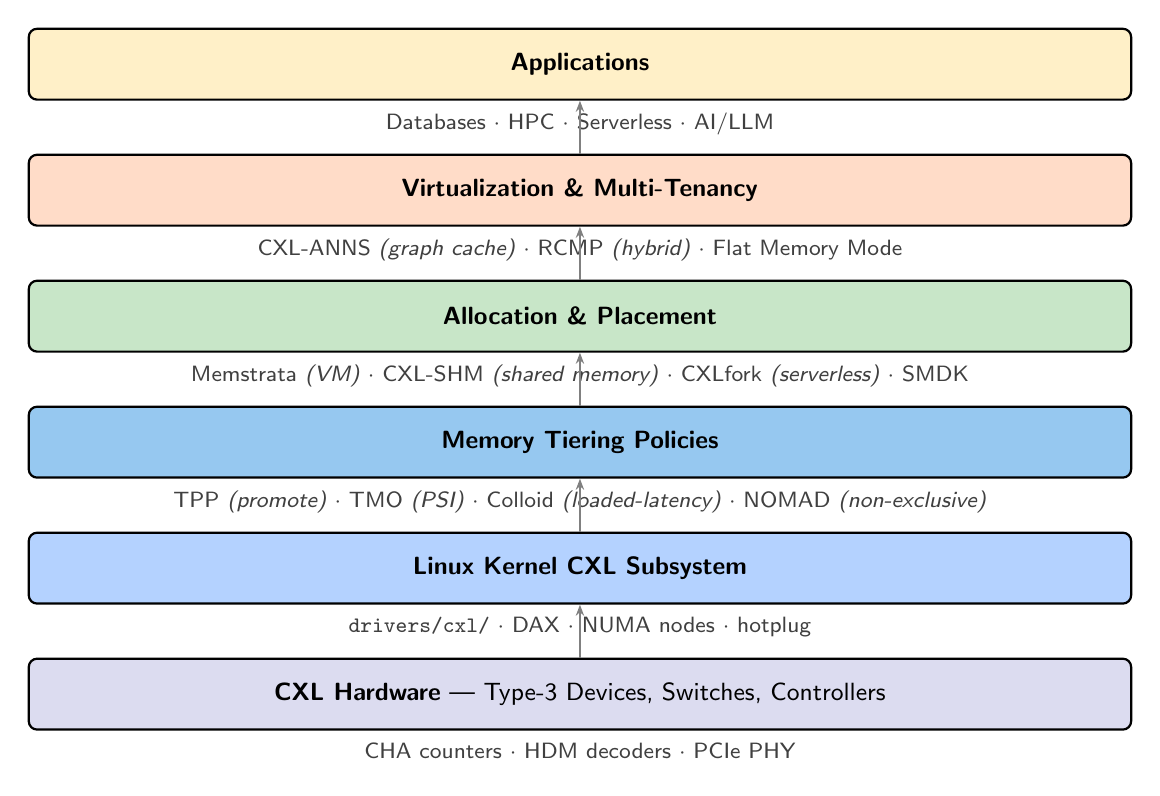
\begin{tikzpicture}[
    layer/.style={draw, rectangle, rounded corners=3pt, minimum height=0.9cm,
                  text centered, font=\sffamily\small, thick, minimum width=14cm},
    work/.style={font=\sffamily\footnotesize, text=gray!50!black},
    sep/.style={draw=none, minimum height=0.15cm},
]

% Color definitions
\definecolor{hwC}{RGB}{220,220,240}
\definecolor{kernC}{RGB}{180,210,255}
\definecolor{tierC}{RGB}{150,200,240}
\definecolor{allocC}{RGB}{200,230,200}
\definecolor{virtC}{RGB}{255,220,200}
\definecolor{appC}{RGB}{255,240,200}

% Layers bottom to top
\node[layer, fill=hwC] (hw) at (0, 0)
  {\textbf{CXL Hardware} --- Type-3 Devices, Switches, Controllers};
\node[work, below=1pt of hw] {CHA counters $\cdot$ HDM decoders $\cdot$ PCIe PHY};

\node[layer, fill=kernC] (kern) at (0, 1.6)
  {\textbf{Linux Kernel CXL Subsystem}};
\node[work, below=1pt of kern] {\texttt{drivers/cxl/} $\cdot$ DAX $\cdot$ NUMA nodes $\cdot$ hotplug};

\node[layer, fill=tierC] (tier) at (0, 3.2)
  {\textbf{Memory Tiering Policies}};
\node[work, below=1pt of tier]
  {TPP \emph{(promote)} $\cdot$ TMO \emph{(PSI)} $\cdot$ Colloid \emph{(loaded-latency)} $\cdot$ NOMAD \emph{(non-exclusive)}};

\node[layer, fill=allocC] (alloc) at (0, 4.8)
  {\textbf{Allocation \& Placement}};
\node[work, below=1pt of alloc]
  {Memstrata \emph{(VM)} $\cdot$ CXL-SHM \emph{(shared memory)} $\cdot$ CXLfork \emph{(serverless)} $\cdot$ SMDK};

\node[layer, fill=virtC] (virt) at (0, 6.4)
  {\textbf{Virtualization \& Multi-Tenancy}};
\node[work, below=1pt of virt]
  {CXL-ANNS \emph{(graph cache)} $\cdot$ RCMP \emph{(hybrid)} $\cdot$ Flat Memory Mode};

\node[layer, fill=appC] (app) at (0, 8.0)
  {\textbf{Applications}};
\node[work, below=1pt of app]
  {Databases $\cdot$ HPC $\cdot$ Serverless $\cdot$ AI/LLM};

% Arrows
\foreach \a/\b in {hw/kern, kern/tier, tier/alloc, alloc/virt, virt/app} {
  \draw[-{Stealth[length=4pt]}, gray, thick] (\a) -- (\b);
}

\end{tikzpicture}
\caption{Taxonomy of systems software for CXL tiered memory management. Each layer builds upon the one below, from hardware telemetry through kernel abstractions to application-level policies. Representative systems are mapped to their primary layer. Works in Section~\ref{sec:software} span the middle four layers.}
\label{fig:sw_stack}
\end{figure*}


\subsection{Evolution of Memory Tiering and Placement}
\label{sec:sw-tiering}

\subsubsection{TPP: First CXL-Aware Kernel Tiering}

Transparent Page Placement (TPP) by Maruf et al.\ was the first CXL-aware memory management feature added to the Linux kernel (version 5.18)~\cite{marufTPPTransparentPage2023}. When analyzing Meta production workloads, the authors discovered that 55--80\% of allocated memory is cold (not accessed for over 2~minutes) and that anonymous pages are much hotter than file-backed pages. TPP introduces four main mechanisms: (1)~lightweight demotion that moves rather than swaps cold pages to CXL memory, (2)~separate allocation and demotion thresholds to keep room for hot allocations, (3)~page-fault-driven promotion that moves hot CXL pages back to local DRAM, and (4)~first-touch allocation bias that directs new anonymous pages to local DRAM, since they are typically short-lived and frequently accessed.

\subsubsection{TMO: Production-Scale Memory Offloading}

Meta's Transparent Memory Offloading (TMO) takes a different approach by adding Pressure Stall Information (PSI)---a kernel feature that measures lost work due to resource shortages---as feedback for memory tiering choices~\cite{10.1145/3503222.3507731}. Unlike TPP's page-access tracking, TMO's Senpai agent applies light memory pressure and uses PSI data to decide how much memory to offload without needing prior application knowledge. TMO works with various backends like zswap compressed memory and NVMe SSDs, with CXL as a suitable future tier. Deployed across Meta's entire fleet, TMO leads to significant memory savings while keeping application-level service level objectives (SLOs).

\subsubsection{Colloid: Loaded-Latency Aware Tiering}

Colloid identifies a major issue in current tiering systems: they assume the default memory tier has lower access latency than other tiers, which is not true under realistic conditions~\cite{10.1145/3694715.3695968}. The authors show that the loaded latency of the default tier can increase by up to five times, making it 2.5 times slower than CXL memory during heavy access. Colloid introduces the idea of \textit{balancing loaded latencies} across tiers using hardware CHA counters and Little's Law to assess each tier's queue occupancy with microsecond precision. When integrated with existing tiering systems like TPP, Colloid achieves a 1.2 to 2.3 times improvement over unchanged baselines.

\subsubsection{Nomad: Non-Exclusive Tiering}

NOMAD challenges the standard exclusive placement model where pages exist in either fast or slow memory~\cite{298669}. Under memory pressure, exclusive tiering can cause excessive swapping of hot pages between tiers. NOMAD keeps shadow copies of promoted pages in CXL memory, allowing efficient demotion by simply changing page table entries for clean pages. Its Transactional Page Migration (TPM) feature copies page content without unmapping the original page, verifying cleanliness upon completion. This means migration does not interfere with the application's critical path and decreases perceived bandwidth loss from as much as 95\% to virtually zero.


\subsection{CXL-Aware Allocation Strategies}
\label{sec:sw-alloc}

\subsubsection{Fine-Grained Placement with Memstrata}

Zhong et al.\ address CXL memory management in cloud virtualization settings with Memstrata~\cite{298671}. The system uses Intel's Flat Memory Mode---a hardware-managed tiering method working at cache-line detail within the memory controller---combined with page coloring to minimize inter-VM contention. A simple online random forest classifier estimates per-VM slowdown from CXL placement, enabling real-time allocation of dedicated local DRAM to performance-sensitive tenants. Across 115 production workloads from Microsoft Azure, Memstrata limits the average VM slowdown to under 5\%.

\subsubsection{Handling Partial Failures}

Zhang et al.\ handle automatic memory management in CXL shared memory during partial failures~\cite{10.1145/3600006.3613135}. Their CXL-SHM system implements era-based non-blocking reference counting, allowing recovery from client crashes without blocking other participants. CXL-SHM achieves tens of millions of allocations per second (43.2 million operations per second) with an asynchronous recovery rate of 23.5 million objects per second.

\subsubsection{Dynamic Forking with CXLfork}

CXLfork showcases a new use for CXL shared memory in serverless computing, enabling zero-copy remote forking across different physical hosts linked through a CXL switch~\cite{10.1145/3676641.3715988}. By keeping process memory in CXL-attached DRAM, CXLfork eliminates the need to transfer memory state during fork operations. This leads to 2.26$\times$ faster cold starts compared to CRIU-based checkpointing, with an 87\% reduction in memory usage. Under memory pressure, CXLfork's companion system CXLporter cuts P99 latency by up to 16$\times$.


\subsection{Virtualization and Multi-Tenancy}
\label{sec:sw-virt}

CXL memory pooling presents distinct virtualization challenges. CXL-ANNS showed that billion-scale vector searches over a shared memory pool need relationship-aware graph caching, keeping nodes within 2--3 hops of the entry point in local DRAM while the rest remains in CXL memory, servicing 59.4\% of traversals locally~\cite{jang2023cxl}. Samsung's SMDK offers a user-space toolkit for explicit CXL memory allocation, including mmap extensions and NUMA-aware placement APIs~\cite{SamsungSMDK2021}. RCMP bridges the transition from RDMA to CXL by combining CXL's low-latency intra-rack access with RDMA's cross-rack scalability in a hybrid setup~\cite{10.1145/3634916}.


%% ============================================================
%% SECTION 5: APPLICATIONS
%% ============================================================
\section{Applications of CXL Type-3 Devices}
\label{sec:apps}

\subsection{In-Memory Databases and Transaction Processing}
\label{sec:app-db}

\subsubsection{Tigon: CXL Pod-Based Distributed Databases}

Tigon introduces the idea of a ``CXL Pod,'' which is a closely connected group of 8 to 16 hosts sharing CXL memory through a multi-headed device (MHD). This serves as a new scaling option for distributed databases~\cite{huang2025tigon}. Within a Pod, Tigon replaces the traditional two-phase commit (2PC) with atomic operations on shared CXL memory. It keeps the Cross-host Active Tuples (CAT, $\sim$7\,MB)---which are the set of tuples accessed concurrently by transactions from different hosts---in CXL memory to avoid network round-trips. The system supports both hardware coherence (HWcc) and software coherence (SWcc) modes. In TPC-C benchmarks, Tigon achieves 2.5 times the throughput compared to shared-nothing baselines and 15.9 to 18.5 times the throughput compared to RDMA-based systems.

\subsubsection{CtXnL: Hybrid Coherence for Transactional Workloads}

Wang et al.\ propose CtXnL, which uses different coherence policies based on data semantics: strict hardware coherence for metadata (locks, indexes) and relaxed software coherence for data records~\cite{10.1145/3676641.3716244}. This hybrid method achieves 2.08 times the throughput of standard CXL coherence while reducing coherence traffic by 95\%.

\subsubsection{PolarCXLMem: Production-Scale Unified Buffer Pool}

PolarCXLMem is the first production deployment of CXL~2.0 switches for cloud-native databases at Alibaba~\cite{10.1145/3722212.3724460}. The system stores the entire database buffer pool (data pages and metadata) in CXL memory, eliminating local buffer management and reducing memory overhead by 30 to 50\%. In pooling scenarios, PolarCXLMem achieves 3.6\,M QPS compared to 1.1\,M QPS for RDMA baselines (3.27$\times$ improvement). Crash recovery is 4.1 to 4.9 times faster because CXL memory's independent power domain preserves buffer state during compute node failures.

% Also: NEW4 SAP HANA \cite{ahn2024examination}, S10 CXL-ANNS \cite{jang2023cxl}


\subsection{HPC, Graph, and Serverless Computing}
\label{sec:app-hpc}

\subsubsection{PMem Migration Pathways in HPC}

With Intel Optane persistent memory discontinued, Fridman et al.\ assess CXL memory as a replacement for PMem-based HPC workloads~\cite{10.1145/3624062.3624175}. STREAM benchmark results show that CXL memory offers comparable bandwidth to Optane PMem while providing better latency predictability. This positions CXL as a natural successor for memory capacity-sensitive HPC applications.

\subsubsection{CXLfork for Serverless Cold Start Acceleration}

In addition to its systems software contribution (Section~\ref{sec:sw-alloc}), CXLfork shows a strong application-level benefit for serverless computing~\cite{10.1145/3676641.3715988}. Function-as-a-Service platforms face multi-second cold start latencies mostly due to memory initialization. CXLfork's zero-copy remote fork cuts cold start times by 2.26$\times$ compared to CRIU while reducing the memory used per function by 87\% through memory sharing across CXL-connected hosts.


\subsection{AI and LLM-Specific CXL Architectures}
\label{sec:app-ai}

\subsubsection{SmartQuant: Bit-Plane Storage for Dynamic Quantization}

SmartQuant uses CXL Type-3 memory as a model store with runtime quantization capability~\cite{10663202}. It organizes model weights in bit-plane format across CXL memory and employs logical space bloating to fit quantized access patterns. This allows for dynamic precision selection at inference time without needing to reload the model.

\subsubsection{CXL-PNM and CLAY: Near-Memory Processing for AI}

CLAY introduces a CXL-based Near-Data Processing architecture for accelerating embedding layers in recommender systems and graph neural networks~\cite{10.1145/3650200.3656595}. Unlike DIMM-based NDP approaches that are limited by memory channel constraints, CLAY uses CXL's packetized protocol to connect DRAM clusters through board-level interconnects, each containing vector processing units alongside memory. This setup allows for detailed load balancing across embedding dimensions while complying with the CXL protocol. CXL-PNM extends this idea to LLM attention and activation computation, offloading memory-heavy tasks to processing elements within CXL expanders~\cite{10476443}.

\subsubsection{Engram as a Co-Design Case Study}

Engram offers compelling evidence that CXL and memory-augmented AI architectures work well together~\cite{chengConditionalMemoryScalable2026}. Engram implements ``conditional memory,'' which adds a sparsity aspect that complements MoE's conditional computation. It retrieves static knowledge patterns through hash-based lookups into large embedding tables (100B+ parameters). Three aspects make this workload ideal for CXL, as shown in Fig.~\ref{fig:ai_cxl}:

\textit{Deterministic addressing}: Unlike attention-based memory access, Engram's N-gram hash lookups generate known addresses before the data is needed, allowing the CPU hardware prefetcher to overlap CXL latency with computation.

\textit{Zipfian locality}: Engram's access pattern follows a power-law distribution where about 10 to 20\% of entries account for over 80\% of accesses. This active set fits in local DRAM or CXL DRAM, while the longer tail is in lower-cost storage.

\textit{Coherence-friendly reads}: The embedding tables are mostly read during inference. This reduces cache invalidation overhead and makes CXL's hardware coherence protocol essentially free compared to RDMA's software-managed consistency.

Engram shows that offloading a 100B-parameter table to host memory results in less than 3\% loss in inference throughput~\cite{chengConditionalMemoryScalable2026}. Since CXL offers a faster and larger memory tier than NVMe, this overhead would decrease further while allowing for cross-node parameter sharing via CXL pooling. Engram's U-shaped scaling law indicates that mixed allocation of around 75 to 80\% MoE computation and 20 to 25\% Engram memory performs better than pure MoE. This suggests that expanding memory capacity with CXL could fundamentally change the compute-memory trade-off in LLM scaling.



%% ---- FIGURE 4: AI & CXL Co-Design (double-column) ----
\begin{figure*}[t]
\centering
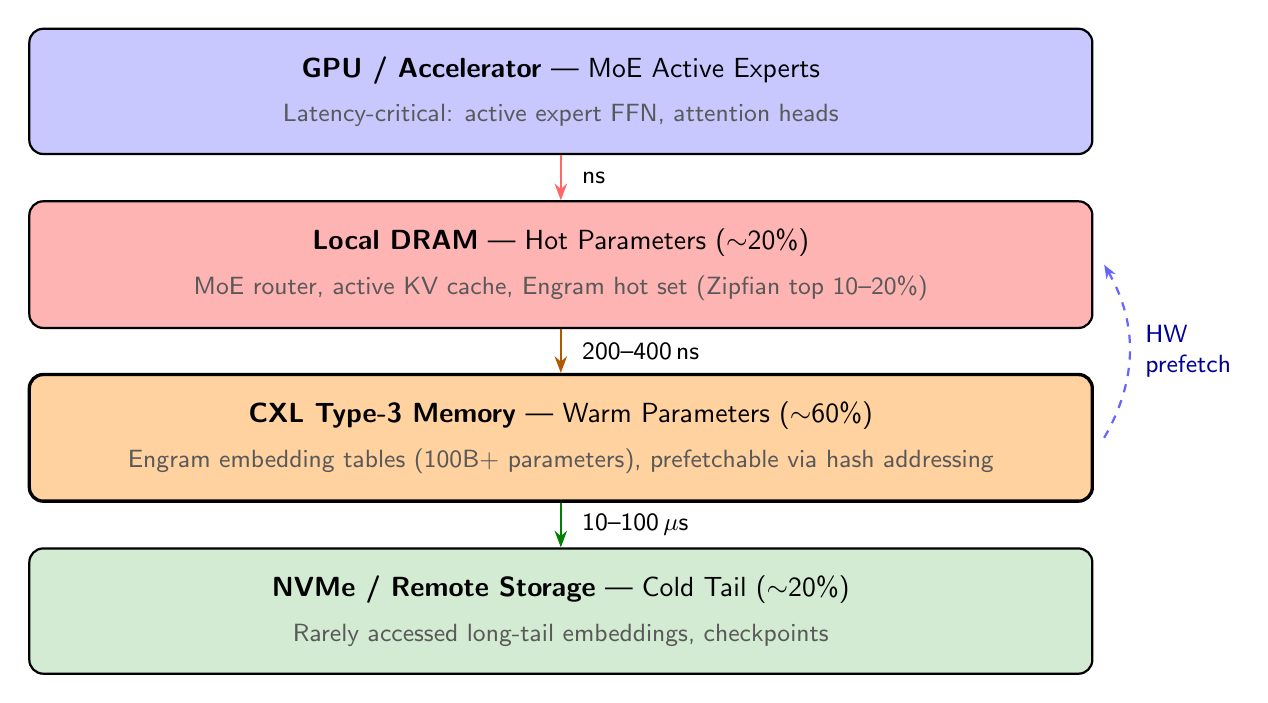
\begin{tikzpicture}[
    % 【修改点1】增加了 inner sep=10pt 让边距拉宽,去掉了固定的高度限制,让文本自动撑开方框
    % 【修改点2】基础字体从 \small 放大为 \normalsize
    block/.style={draw, rectangle, rounded corners=5pt, thick,
                  font=\sffamily\normalsize, align=center, 
                  minimum width=13.5cm, inner sep=10pt},
    % 稍微放大了箭头尺寸
    arrow/.style={thick, -{Stealth[length=6pt]}},
    speed/.style={font=\sffamily\small, text=black}
]

\definecolor{gpuC}{RGB}{200,200,255}
\definecolor{hotC}{RGB}{255,180,180}
\definecolor{warmC}{RGB}{255,210,160}
\definecolor{coldC}{RGB}{210,235,210}

% 【修改点3】拉开了整体的Y轴间距(6.6, 4.4, 2.2, 0),并且将原先在外部的 anno 文本合并到了方框内(使用 \\[4pt] 换行)

% GPU / Compute
\node[block, fill=gpuC] (gpu) at (0, 6.6)
  {\textbf{GPU / Accelerator} --- MoE Active Experts\\[4pt]
   \textcolor{gray!70!black}{\small Latency-critical: active expert FFN, attention heads}};

% Local DRAM = Hot tier
\node[block, fill=hotC] (hot) at (0, 4.4)
  {\textbf{Local DRAM} --- Hot Parameters ($\sim$20\%)\\[4pt]
   \textcolor{gray!70!black}{\small MoE router, active KV cache, Engram hot set (Zipfian top 10--20\%)}};

% CXL Memory = Warm tier
\node[block, fill=warmC, line width=1.2pt] (warm) at (0, 2.2)
  {\textbf{CXL Type-3 Memory} --- Warm Parameters ($\sim$60\%)\\[4pt]
   \textcolor{gray!70!black}{\small Engram embedding tables (100B+ parameters), prefetchable via hash addressing}};

% NVMe = Cold tier
\node[block, fill=coldC] (cold) at (0, 0)
  {\textbf{NVMe / Remote Storage} --- Cold Tail ($\sim$20\%)\\[4pt]
   \textcolor{gray!70!black}{\small Rarely accessed long-tail embeddings, checkpoints}};

% Arrows between tiers (现在箭头在方框之间干干净净,不会穿透文字了)
\draw[arrow, red!60] (gpu) -- (hot) node[midway, right=4pt, speed] {ns};
\draw[arrow, orange!70!black] (hot) -- (warm) node[midway, right=4pt, speed] {200--400\,ns};
\draw[arrow, green!50!black] (warm) -- (cold) node[midway, right=4pt, speed] {10--100\,$\mu$s};

% Prefetch annotation (将坐标调整到方框右侧外边缘 6.9 的位置)
\draw[-{Stealth[length=5pt]}, dashed, blue!60, thick]
  (6.9, 2.2) to[bend right=30] node[midway, right=2pt, font=\sffamily\small, text=blue!60!black, align=left] {HW\\prefetch} (6.9, 4.4);

\end{tikzpicture}
\caption{Memory mapping strategy for LLMs on CXL tiered memory. Latency-critical compute parameters (active MoE experts) reside in GPU/accelerator memory, while Engram's massive embedding tables---whose Zipfian access patterns and deterministic hash addressing enable effective hardware prefetching---are offloaded to CXL Type-3 memory. The long tail migrates to NVMe storage. (Adapted from insights in~\cite{chengConditionalMemoryScalable2026}.)}
\label{fig:ai_cxl}
\end{figure*}



\begin{table}[t]
\centering
\caption{Comparison of Interconnect Technologies for Sparse Parameter Access}
\label{tab:interconnect-comparison}
\begin{tabular}{lccc}
\toprule
\textbf{Dimension} & \textbf{CXL.mem} & \textbf{RDMA} & \textbf{NVMe} \\
\midrule
Latency & 200--400\,ns & 2--5\,$\mu$s & 10--100\,$\mu$s \\
Addressing & Byte, load/store & Page, verbs & Block, I/O \\
Coherence & HW cache coherent & None & None \\
Prefetch & CPU prefetcher & No & No \\
\bottomrule
\end{tabular}
\end{table}


%% ============================================================
%% SECTION 6: OPEN CHALLENGES
%% ============================================================
\section{Open Challenges and Future Directions}
\label{sec:challenges}

\subsection{Protocol Bottlenecks and Tail Latency}
\label{sec:ch-latency}

Although CXL reduces the gap between local and remote memory, tail latency remains a major issue. Liu et al.\ found that CXL tail latency increases significantly under contention, with bandwidth-bound workloads experiencing slowdowns of 1.5 to 5.8 times, while CXL+NUMA configurations can lead to up to 2.9$\times$ degradation, even with low bandwidth demands~\cite{10.1145/3676641.3715987}. The 256-byte flit overhead and protocol processing add fixed latency that becomes increasingly significant for small random accesses. CXL~4.0's bandwidth increase to 128\,GT/s should help with throughput bottlenecks~\cite{CXL4.0}, but managing tail latency needs workload-aware placement policies and possibly hardware-level QoS mechanisms that are not yet in the specification.


\subsection{Security and Isolation}
\label{sec:ch-security}

Shared CXL memory pools create new vulnerabilities. Two recent studies tackle this challenge from different perspectives.

\subsubsection{CXL-Address-Based Security}

Abdullah et al.\ propose Salus, a security model for systems with dynamic page migration between GPU memory and CXL-expanded pools~\cite{10476444}. Salus separates security metadata from physical data locations, which minimizes costly security recalculations during page migration. The evaluation shows a geometric mean improvement of 29.94\% in GPU throughput compared to traditional security models, with security-related traffic reduced to 47.79\% of baseline levels.

\subsubsection{Scalable Freshness Guarantees with Toleo}

Dong et al.\ introduce Toleo, which uses a small CXL-attached smart memory device (168\,GB) with Processing-in-Memory (PIM) capability to safeguard a larger 28\,TB CXL pool~\cite{10.1145/3622781.3674180}. Toleo achieves a 240$\times$ metadata compression ratio through trip-based version tracking, keeping freshness guarantees with only 2\% performance overhead. The system uses CXL IDE (Integrity and Data Encryption) for in-transit protection.


\subsection{AI-Systems Co-Design: The Engram Case}
\label{sec:ch-codesign}

Combining memory-augmented AI designs with CXL infrastructure offers a unique co-design chance. Engram's conditional memory concept~\cite{chengConditionalMemoryScalable2026} shows that AI model designers can shape memory access patterns to fit CXL features. Future co-design could cover three areas: \textit{hardware} (CXL controllers with application-aware prefetch logic), \textit{operating systems} (workload-specific tiering policies for AI memory access patterns), and \textit{model architecture} (designing memory layers that consider CXL latency and bandwidth limits).


\subsection{Future Directions}
\label{sec:ch-future}

Several emerging trends will influence CXL Type-3 adoption. Near-memory computing, as shown by CLAY's NDP approach~\cite{10.1145/3650200.3656595}, shifts computation to CXL expanders to lower data movement. The merger of CXL~4.0 with UCIe (Universal Chiplet Interconnect Express) promises closer integration of memory and compute chiplets. Multi-rack CXL fabrics, now supported in CXL~4.0~\cite{CXL4.0}, will enable memory pooling at the datacenter level. Lastly, the CXL software ecosystem is still developing: standardized benchmarking suites, production-quality drivers for compatibility with different vendors, and application-level profiling tools are essential gaps that need to be filled for broader adoption.


%% ============================================================
%% SECTION 7: CONCLUSION
%% ============================================================
\section{Conclusion}
\label{sec:conclusion}

This survey has looked into CXL Type-3 devices regarding hardware, systems software, and applications, addressing four research questions.

\textbf{RQ1 (Performance):} Real CXL hardware adds 200 to 400\,ns latency compared to local DRAM, with bandwidth reaching 40\,GB/s for sequential reads. Performance varies widely among implementations, and NUMA emulation tends to overstate CXL overhead.

\textbf{RQ2 (Systems Software):} Memory tiering has progressed from basic page-fault-driven promotion (TPP) to large-scale offloading (TMO), then to contention-aware placement (Colloid) and non-exclusive caching (NOMAD). Each method addresses increasingly detailed aspects of CXL memory management.

\textbf{RQ3 (Applications):} Databases are the primary beneficiaries, with production implementations at Alibaba (PolarCXLMem) showing 3.27$\times$ throughput gains. HPC and serverless workloads benefit from CXL's larger capacity and zero-copy forking. The AI sector, though still in early stages, shows great long-term promise because memory-augmented architectures have access patterns that fit well with CXL features.

\textbf{RQ4 (Challenges):} Managing tail latency, ensuring security in shared pools, and maturing the software ecosystem remain key hurdles. The most promising opportunity lies in co-designing hardware, software, and models, where CXL-aware AI architectures could greatly change the compute-memory trade-off.

CXL Type-3 devices are more than just faster memory expanders; they represent a fundamental shift in how datacenter systems manage and share memory resources. As CXL~4.0 enables multi-rack fabrics and near-memory computing, the systems and AI communities must work together to fully realize this potential.


%% ============================================================
%% REFERENCES
%% ============================================================
% Bibliography (pre-compiled .bbl for arXiv)
\bibliographystyle{IEEEtran}
\bibliography{references}

\end{document}
